% % 3-felder.te
%
% (c) 2024 Prof Dr Andreas Müller
%
\section{Erhaltungssätze für Felder
\label{buch:symmetrien:felder}}
\kopfrechts{Erhaltungssätze für Felder}
Für Felder im Gegensatz zu Funktionen einer Variablen muss der
Begriff einer Symmetrie neu formuliert werden und auch der Begriff
eines Erhaltungssatzes muss angepasst werden.
Das Konzept der Divergenz eines Vektorfeldes
und die Kontinuitätsgleichung sind der Ausgangspunkt.
Dieser Abschnitt folgt der Darstellung in \cite[section 8.6]{buch:pde}.

%
% Divergenzform
%
\subsection{Divergenzform
\label{buch:symmetrien:felder:subsection:divergenzform}}
Wir versuchen erst zu ermitteln, welche Art von Gleichung wir anstelle
einer Konstanten als Erhaltungssatz erwarten dürfen.

%
% Kontinuitätsgleichung
%
\subsubsection{Kontinuitätsgleichung}
Wir betrachten die Dichteverteilung $\varrho(x,y,z,t)$ eines Mediums
im dreidimensionalen Raum zusammen mit dem Vektorfeld $\vec{v}(x,y,z,t)$
der Strämungsgeschwindigkeit.
Dann können wir in einem kleinen Quader mit Seitenlägen
$\Delta x$,
$\Delta y$
und
$\Delta z$
die Veränderung der darin enthaltenen Masse auf zwei Arten berechnen.
Einerseits wird sie approximiert durch die Änderung der Dichte
\[
\Delta m
=
\bigl(\varrho(x,y,z,t+\Delta t)-\varrho(x,y,z,t)\bigr)
\Delta x
\,
\Delta y
\,
\Delta z.
\]
Andererseits kann man die durch die Seitenflächen fliessenden Masse
ermitteln.
Der Massestrom ist das Produkt $\vec{\jmath}=\varrho\vec{v}$.
Damit wird
\begin{align*}
\Delta m
&=
\bigl(
j_x(x+\Delta x,y,z,t)
-
j_x(x,y,z,t)
\bigr)
\Delta y\,\Delta z \, \Delta t
\\
&\quad
+
\bigl(
j_y(x,y+\Delta y,z,t)
-
j_y(x,y,z,t)
\bigr)
\Delta x\,\Delta z \, \Delta t
\\
&\quad
+
\bigl(
j_z(x,y,z+\Delta z,t)
-
j_z(x,y,z,t)
\bigr)
\Delta x\,\Delta y \, \Delta t
\end{align*}
Nach Division durch $\Delta x\, \Delta y\, \Delta z\,\Delta t$ ergeben
die Terme die Gleichung
\begin{align*}
\frac{\Delta m}{\Delta x\,\Delta y\,\Delta z\,\Delta t}
&=
\frac{\varrho(x,y,z,z+\Delta t)-\varrho(x,y,z,t)}{\Delta t}
\\
&=
\frac{
j_x(x+\Delta x,y,z,t)
-
j_x(x,y,z,t)
}{
\Delta x
}
\\
&\quad
+
\frac{
j_y(x,y+\Delta y,z,t)
-
j_y(x,y,z,t)
}{
\Delta y
}
\\
&\quad
+
\frac{
j_z(x,y,z+\Delta z,t)
-
j_z(x,y,z,t)
}{
\Delta z
}.
\end{align*}
Nach dem Grenzübergang
$\Delta x\to 0$,
$\Delta y\to 0$,
$\Delta z\to 0$
und
$\Delta t\to 0$
wird daraus die Kontinuitätsgleichung
\index{Kontinuitätsgleichung}%
\begin{equation}
\frac{\partial \varrho}{\partial t}(x,y,z,t)
=
\frac{\partial j_x}{\partial x}(x,y,z,t)
+
\frac{\partial j_y}{\partial y}(x,y,z,t)
+
\frac{\partial j_z}{\partial 7}(x,y,z,t)
=
\operatorname{div}\vec{\jmath}(x,y,z,t).
\label{buch:symmetrien:felder:eqn:kontinuitaet}
\end{equation}
Die Kontinuitätsgleichung ist der prototypische Erhaltungssatz für
Felder.
Beispielsweise ist die Wärmeleitungsgleichung nur die Kontinuitätsgleichung
für die Wärmeenergiedichte und den Wärmeenergiestrom.
\index{Wärmeenergiedichte}%
\index{Wärmeleitungsgleichung}%

%
% Divergenzform
%
\subsubsection{Divergenzform}
\index{Divergenzform}%
Wenn eine skalare Grösse wie die Dichte $\varrho$ erhalten ist, dann bleibt
in der zugehörigen Kontinuitätsgleichung mit der Stromdichte
$\vec{\jmath}$ nur die rechte Seite stehen, es gilt dann
\[
\frac{\partial\varrho}{\partial t}
=
0
=
\operatorname{div} \vec{\jmath}.
\]
Anstelle einer Grösse, die konstant bleibt, kann man daher nur erwarten,
dass es ein Vektorfeld gibt, dessen Divergenz verschwindet.

%
% Gebietsvariation und Multiplikator
%
\subsection{Gebietsvariation und Multiplikator}
Bei der Variation einer Funktion der Variablen $t$ kann sich das
Definitionsgebiet nur dadurch ändern, dass die Endpunkte des
Definitionsintervalls verschoben werden.
Dies kann durch zwei Funktionen $t_0(s)$ und $t_1(s)$ beschrieben werden.
Für eine Funktion von mehreren Variablen wird das Problem komplizierter,
da das Definitionsgebiet eine beliebige offene Teilmenge von $\mathbb{R}^n$
sein kann.
Allerdings soll sich auch der Zusammenhang des Gebietes nicht ändern,
es sollen also bei der Deformation keine neuen Randstücke oder ``Löcher''
entstehen.
Wir definieren daher eine Gebietsvariation wie folgt.

\begin{definition}
Eine differenzierbare Abbildung
\[
\varphi^s
\colon
\mathbb{R}^n\times \mathbb{R}
:
(x,s)
\mapsto
\varphi^s(x),
\qquad
\varphi^0(x)=x
\]
heisst eine {\em Gebietsvariation}.
\index{Gebietsvariation}%
Die Ableitung
\[
\frac{\partial \varphi^s(x)}{\partial s}\bigg|_{s=0}
=
\vec{v}(x)
\]
nach $s$ an der Stelle $s=0$ ist ein $n$-dimensionales Vektorfeld.
\end{definition}

%
% fig-rand.tex
%
% (c) 2024 Prof Dr Andreas Müller
%
\begin{figure}
\centering
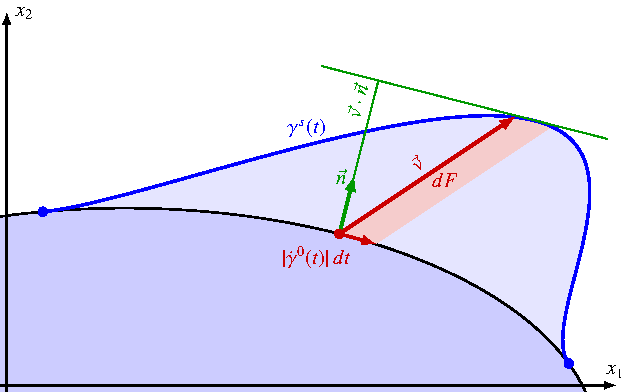
\includegraphics{chapters/100-symmetrien/images/rand.pdf}
\caption{Zum Beweis des
Satzes~\ref{buch:symmetrien:felder:satz:gebietsintegral}:
Änderung eines Integrals bei Verschiebung des Randes.
\label{buch:symmetrien:felder:fig:rand}}
\end{figure}
%

\begin{satz}
\label{buch:symmetrien:felder:satz:gebietsintegral}
Für eine $f\colon \mathbb{R}^n\to\mathbb{R}$ differenzierbare Funktion
gilt
\begin{equation}
\frac{d}{ds}
\int_{\varphi^s(U)}
f(x)\,dx
\bigg|_{s=0}
=
\int_{\partial U} f(x)\vec{v}(x)\cdot d\vec{o}.
\label{buch:symmetrien:felder:eqn:gebietsintegral}
\end{equation}
\end{satz}

\begin{proof}[Beweisskizze]
Wir beschränken uns auf eine Skizze für den Fall $n=2$, sie lässt
sich leicht zu einem vollen Beweis für beliebiges $n$ ausbauen.

Die Veränderung des Gebiets entsteht durch Verschiebung des Randes,
den wir als Kurve $\gamma^s(t)$ parametrisieren 
Abbildung~\ref{buch:symmetrien:felder:fig:rand}).
Wir nehmen der Einfachheit halber an, dass sich die Verschiebung des
Randes auf das Intervall $[a,b]$ beschränkt, dass also
$\gamma^s(a)=\operatorname{const}$
und
$\gamma^s(b)=\operatorname{const}$
ist.
Da es in \eqref{buch:symmetrien:felder:eqn:gebietsintegral}
nur um die Ableitung geht, ist nur die Verschiebung des Randes 
in erster Ordnung wichtig.
Wir können daher die Verschiebung durch
\[
\gamma^s(t) 
=
\gamma^0(t)
+
s \frac{\partial \gamma^s}{\partial s}(t) \bigg|_{s=0}
+ o(s)
=
\gamma^0(t)
+
s\vec{v}(\gamma^0(t))
+
o(s)
\]
beschreiben.
Die Variablen $s$ und $t$ beschreiben ein Koordinatensystem in der
Nähe des Randes, mit dem das Integral in der Nähe es Randes ausgewertet
werden kann.

In jedem Punkt $\gamma^0(t)$ des Randes sei $\vec{n}(t)$ die nach
aussen zeigende Normale.
Wenn der Rand um $s\vec{v}(\gamma^0(t))$ verschoben wird,
ändert sich sein Abstand vom Rand um 
$s\vec{v}(\gamma^0(t))\cdot \vec{n}(t)$.
Der Rand für Parameterwerte zwischen $t$ und $t+dt$ überstreicht
daher in Parallelogramm mit Flächeninhalt
\[
dF
=
s\vec{v}(\gamma^0(t))\cdot \vec{n}(t)
\,
|\dot{\gamma(t)}|
\,dt.
\]

Das Veränderung des Gebietsintegrals durch die Verschiebung des
Randes ist daher in erster Ordnung durch
\begin{align*}
\int_{\varphi^s(U)} f(x)\,dx
&=
\int_{\varphi^0(U)} f(x)\,dx
+
\int_a^b
f(\gamma(t))
\,dF
\\
&=
\int_{\varphi^0(U)} f(x)\,dx
+
s
\int_a^b
f(\gamma(t))
\,
\vec{v}(\gamma^0(t))
\cdot \vec{n}(t)
\,
|\dot{\gamma}^0(t)|
\,dt
+
o(s)
\end{align*}
gegeben.
Für die Ableitung folgt daher das Integral
\begin{align*}
\frac{d}{ds}
\int_{\varphi^s(U)} f(x)\,dx\,\bigg|_{s=0}
&=
\int_a^b
f(\gamma^0(t))
\,
\vec{v}(\gamma^0(t)) \cdot \vec{n}(t)
\,
|\dot{\gamma}^0(t)|\,dt
\\
&=
\int_{\partial U}
f(x)
\,
\vec{v}(x) \cdot
d\vec{n}.
\end{align*}
Dies ist das Integral des Flusses des Vektorfeldes 
\[
f(x)  \vec{v}(x),\qquad x\in\partial U,
\]
durch den Rand des Gebietes.
Damit ist der Satz in diesem Spezialfall bewiesen.
\end{proof}

\begin{definition}
Die {\em allgemeine Variation} einer Funktion
\index{allgemeine Variation}%
\(
u
\colon
\mathbb{R}^n\to \mathbb{R}
\)
ist eine Funktion
\[
w
\colon
\mathbb{R}^n \times\mathbb{R}
\to
\mathbb{R}
:
(x,s)
\mapsto
w(x,s)
\]
mit $w(x,0)=u(x)$.
Die Ableitung
\[
\frac{\partial w}{\partial s}(x,0) = m(x)
\]
nach $s$ an der Stelle $s=0$ heisst ein {\em Multiplikator}.
\index{Multiplikator}%
\end{definition}

\begin{definition}
Ein Funktional mit Lagrange-Funktioin
$L(x,u,u_x)$ heisst unter der Gebietsvariation $\varphi^s$ und
der allgemeinen Variation $w$ von $u$ invariant, wenn
\begin{equation}
\int_U
L(x,w(x,s),\nabla w(x,s))\,dx
=
\int_{\varphi^s(U)}
L(x,u(x),\nabla u(x))\,dx
\label{buch:symmetrien:felder:eqn:invarianz}
\end{equation}
gilt.
\end{definition}

%
% Der Satz von Noether für Felder
%
\subsection{Der Satz von Noether für Felder}
Wenn die Lagrange-Funktion eines Funktionals unter einer Gebietsvariation
und einer allgemeine Variation von $u$ invariant ist, dann gibt es einen
Stromvektor, dessen Divergenz verschwindet.

\begin{satz}
Ist das Funktional $I$ mit Lagrange-Funktion $L$ invariant unter $\varphi^s$
und $w$.
Der Vektor $\vec{j}$ habe die Komponenten
\index{Strom}%
\[
j_k
=
L\bigl(x,u(x),\nabla u(x)\bigr)\,v_k(x)
-
m(x)
\frac{\partial L}{\partial u_{x_k}}\bigl(x,u(x),\nabla u(x)\bigr).
\]
Dann gilt
\begin{align}
\operatorname{div}\vec{\jmath}
=
\sum_{k=1}^n \frac{\partial j_k}{\partial x_k}
&=
\sum_{k=1}^n
\frac{\partial }{\partial x_k}
\biggl(
L\bigl(x,u(x),\nabla u(x)\bigr)\,v_k(x)
-
m(x)
\frac{\partial L}{\partial u_{x_k}}
\bigl(x,u(x),\nabla u(x)\bigr)
\biggr)
\notag
\\
&=
m(x)\biggl(
\frac{\partial L}{\partial u}\bigl(x,u(x),\nabla u(x)\bigr)
-
\sum_{k=1}^n\frac{\partial L}{\partial u_{x_k}}\bigl(x,u(x),\nabla u(x)\bigr)
\biggr)
\label{buch:symmetrien:felder:eqn:rhs}
\end{align}
Falls $u$ ein kritischer Punkt des Funktionals $I$ ist, gilt
\[
\operatorname{div}\vec{\jmath}=0.
\]
\end{satz}

\begin{proof}
Die Klammer auf der rechten Seite von \eqref{buch:symmetrien:felder:eqn:rhs}
ist
\[
E(x)
=
\frac{\partial L}{\partial u}\bigl(x,u(x),\nabla u(x)\bigr)
-
\sum_{k=1}^n\frac{\partial L}{\partial u_{x_k}}\bigl(x,u(x),\nabla u(x)\bigr).
\]
Dies ist die linke Seite der Euler-Ostrogradski-Diffe\-ren\-tial\-gleichung
für die Funktion $u$.
Für einen kritischen Punkt $u$ des Funktionals ist die rechte Seite
von \eqref{buch:symmetrien:felder:eqn:rhs} $=0$,
die letzte Behauptung folgt daher aus~\eqref{buch:symmetrien:felder:eqn:rhs}.

Wir berechnen die Ableitung der
Identität~\eqref{buch:symmetrien:felder:eqn:invarianz}
an der Stelle $s=0$.
Für die linke Seite erhalten wir wegen $w(x,s)=u(x)$
\begin{align*}
\text{LHS}
&=
\int_U
\frac{\partial L}{\partial u}\bigl(x,u(x),\nabla u(x)\bigr)
\frac{\partial w}{\partial s}(x,0)
+
\sum_{k=1}^n
\frac{\partial L}{\partial u_{x_k}}\bigl(x,u(x),\nabla u(x)\bigr)
\cdot
\frac{\partial}{\partial s}
\frac{\partial w}{\partial x_k}(x,0)
\,dx.
\end{align*}
Die Ableitung von $w(x,s)$ nach $s$ ergibt den Multiplikator $m(x)$.
Die beiden Ableitungen von $w$ in der Summe können vertauscht werden
und ebenfalls durch $m(x)$ ausgedrückt werden, nämlich als
\[
\frac{\partial s}{\partial w}{\partial x_k}(x,0)
=
\frac{\partial }{\partial x_k}\frac{\partial w}{\partial s}(x,0)
=
\frac{\partial m}{\partial x_k}(x)
\]
Somit ist
\begin{align*}
\text{LHS}
&=
\int_U
\frac{\partial L}{\partial u}\bigl(x,u(x),\nabla u(x)\bigr)
m(x)
+
\sum_{k=1}^n
\frac{\partial L}{\partial u_{x_k}}\bigl(x,u(x),\nabla u(x)\bigr)
\cdot
\frac{\partial m}{\partial x_k}(x)
\,dx.
\intertext{Partielle Integration der Summe ergibt}
&=
\int_U
\frac{\partial L}{\partial u}\bigl(x,u(x),\nabla u(x)\bigr)
m(x)
\,dx
+
\int_{\partial U}
m(x)
\frac{\partial L}{\partial u_{x}}\bigl(x,u(x),\nabla u(x)\bigr)
\cdot
d\vec{o}
\\
&\qquad
-
\int_{U}
m(x)
\sum_{k=1}^n
\frac{\partial}{\partial x_k}
\frac{\partial L}{\partial u_{x_k}}\bigl(x,u(x),\nabla u(x)\bigr)
\,dx.
\\
&=
\int_U
m(x)
\biggl(
\frac{\partial L}{\partial u}\bigl(x,u(x),\nabla u(x)\bigr)
-
\sum_{k=1}^n
\frac{\partial}{\partial x_k}
\frac{\partial L}{\partial u_{x_k}}\bigl(x,u(x),\nabla u(x)\bigr)
\biggr)\,dx
\\
&\qquad
+
\int_{\partial U}
m(x)
\frac{\partial L}{\partial u_{x}}\bigl(x,u(x),\nabla u(x)\bigr)
\cdot
d\vec{o}
\intertext{oder noch einfacher}
&=
\int_U
m(x)
E(x)
\,dx
+
\int_{\partial U}
m(x)
\frac{\partial L}{\partial u_{x}}\bigl(x,u(x),\nabla u(x)\bigr)
\cdot
d\vec{o}.
\end{align*}

Die rechte Seite der Ableitung der
Identität~\eqref{buch:symmetrien:felder:eqn:invarianz}
wendet die Formel für die Ableitung eines Integrals über ein
von einem Parameter abhängendes Gebiet von
Satz~\ref{buch:symmetrien:felder:satz:gebietsintegral}
auf die Funktion $f(x) = L\bigl(x,u(x),\nabla u(x)\bigr)$ an, die
\[
\frac{d}{ds}
\int_{\varphi^s(U)} L\bigl(x,u(x),\nabla u(x)\bigr)\,dx
\bigg|_{s=0}
=
\int_U L\bigl(x,u(x),\nabla u(x)\bigr)\,\vec{v}\cdot d\vec{o}.
\]
ergibt.

Die bisherigen Rechnungen haben ergeben, dass
\begin{align*}
\int_U m(x) E(x)\,dx
+
\int_{\partial U}
m(x)\frac{\partial L}{\partial u_x}\bigl(x,u(x),\nabla u(x)\bigr)\cdot d\vec{o}
&=
\int_{\partial U}L\bigl(x,u(x),\nabla u(x)\bigr)\,\vec{v}(x)\cdot d\vec{o}.
\end{align*}
Bringen wir das zweite Integral links auf die rechte Seite, ergibt
sich
\begin{align*}
\int_U m(x) E(x)\,dx
&=
\int_{\partial U}
\biggl(
-
m(x)\frac{\partial L}{\partial u_x}\bigl(x,u(x),\nabla u(x)\bigr)
+
\int_{\partial U}L\bigl(x,u(x),\nabla u(x)\bigr)\,\vec{v}(x)
\biggr)
\cdot d\vec{o}.
\intertext{Mit dem Integralsatz von Gauss kann das Oberflächenintegral
auf der rechten Seite in das Gebietsintegral über $U$}
&=
\int_U
\operatorname{div}
\biggl(
L\bigl(x,u(x),\nabla u(x)\bigr)\,\vec{v}(x)
-m(x)
\frac{\partial L}{\partial u_x}\bigl(x,u(x),\nabla u(x)\bigr)
\biggr)
\,dx
\intertext{umgewandelt werden.
In Komponenten ist dies}
&=
\int_U
\sum_{k=1}^n
\frac{\partial}{\partial x_k}
\biggl(
L\bigl(x,u(x),\nabla u(x)\bigr)\,v_k(x)
-m(x)
\frac{\partial L}{\partial u_{x_k}}\bigl(x,u(x),\nabla u(x)\bigr)
\biggr)
\,dx
\intertext{oder}
\int_U m(x) E(x)\,dx
&=
\int_U \sum_{k=1}^n \frac{\partial j_k}{\partial x_k}(x) \,dx
=
\int_U \operatorname{div}\vec{\jmath}\,dx.
\end{align*}
Da dies für jedes beliebige Gebiet $U$ gilt, müssen auch die Integranden
\begin{equation}
m(x)
E(x)
=
\operatorname{div}\vec{\jmath}
\end{equation}
übereinstimmen.
Dies ist die Gleichung \eqref{buch:symmetrien:felder:eqn:rhs}.
Damit ist der Satz bewiesen.
\end{proof}


